\documentclass{IEEEtran}

\usepackage{amsmath}
\usepackage{listings}
\lstset{
    basicstyle=\small\ttfamily,
    breaklines=true
}
\usepackage{graphicx}
\graphicspath{ {./images/} }
\usepackage{xcolor}
\pagecolor[rgb]{0.1,0.1,0.1}
\color[rgb]{1,1,1}

\title{Readings about Strings and Tries}
\author{Diego Linares - kiwiAipom}

\begin{document}
  \maketitle
  \section{Manacher's Algorithm}
    \textbf{Statement:} Find all pairs $(i,j)$ which make a palyndrome substring.
    \subsection{Detailed Statement}
      Worst case we would have $O(n^2)$ palyndromes.\par 
      \textbf{Compact way of keeping palyndromes:} $i = 0\ldots n-1$, $d_1[i],d_2[i]$ represent the number of palyndromes with odd and even length with their center in $i$.\par 
      \textbf{Ex.} $abababc$, has $d_1=3$ (odd length), and $cbaabd$ has $d_2[3] = 2$ (even length). \par 
      Sub-palindrome with $l$ size with center in $i$, we also have with $l-2, l-4,\ldots$. \par 
      Both palyndrom arrays can be calculated in linear time. \par 
      \textbf{Solution:} Can be done with string hashing and suffix trees, but this has a smaller constant and memory complexity.
    \subsection{Trivial Algorithm}
      Tries to increase the answer by one until it's possible for each center $i$. It is $O(n^2)$ in time. Implementation being:
      \begin{lstlisting}
vector<int> d1(n),  d2(n);
for (int i = 0; i < n; i++) {
    d1[i] = 1; // Pair with itself 
    while (0 <= i - d1[i] && i + d1[i] < n && s[i - d1[i]] == s[i + d1[i]]) {
        d1[i]++;
    }

    d2[i] = 0;
    while (0 <= i - d2[i] - 1 && i + d2[i] < n && s[i - d2[i] - 1] == s[i + d2[i]]) {
        d2[i]++;
    }
}
      \end{lstlisting}
    \subsection{Manacher's Algorithm}
      Allows to find all the sub-palyndromes with odd length (even length is just a small mod).\par 
      \textbf{Borders:} $(l,r)$ of the palyndrome with maximal $r$. Initially we assume $l=0,r=-1$\par 
      We want to calculate $d_1[i]$ with all the previous $i$ already calculated.
      \begin{itemize}
        \item If it is ourside of the current rightmost sub-palyndrome $i > r$, we launch the trivial algorithm, allowing us to calculate $d_i[i]$ and updating $(l,r)$.
        \item $i \leq r$. We can flip $i$ into $j=l+(r-i)$ and since they are symmetrical, we can \textbf{almost always} do $d_1[i] = d_1[j]$. Like so: 
        \begin{center}
          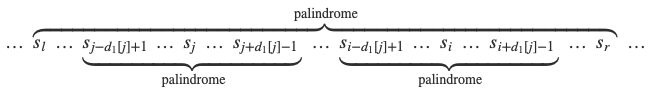
\includegraphics[width = 0.45\textwidth]{manacherIllust.png}
        \end{center}
        \item \textbf{Trick case:} When the inner palyndrome reaches the border of the outer one. $j-d_1[j]+1\leq l$. Since the symmetry of the outer palyndrome is not guaranteed, we assign $d_1[i] = r - i + 1$, and then run the trivial algorithm to increase the value if necessary, updating in the end. Like so:
        \begin{center}
          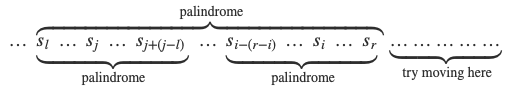
\includegraphics[width=0.45\textwidth]{manacherTrick.png}
        \end{center}
        \par Note we only use the part of the palyndrome with guaranteed symmetry before moving to the \textit{try moving here part}. 
      \end{itemize}
      \par A similar algorithm is then used for the even part.
    \subsection{Complexity}
      Not as intuitive, but if we look at \textit{Z-function building algorithm} we can check it's similar and linear. \par 
      We can also notice that $r$ can only increase by one ine very iteration of the trivial algorithm, and that it can't decrease. $O(n)$ iterations. The rest is linear.
    \subsection{Implementation}
      Here is the implementation, which is fairly similar for both $d_1,d_2$.
      \begin{lstlisting}
vector<int> d1(n), d_2(n);
for (int i = 0, l = 0, r = -1; i < n; i++) {
    int k = (i > r) ? 1 : min(d1[l + r - i], r - i + 1);
    while (0 <= i - k && i + k < n && s[i - k] == s[i + k]) {
        k++;
    }
    d1[i] = k--;
    if (i + k > r) {
        l = i - k;
        r = i + k;
    }
}
for (int i = 0, l = 0, r = -1; i < n; i++) {
    int k = (i > r) ? 0 : min(d2[l + r - i + 1], r - i + 1);
    while (0 <= i - k - 1 && i + k < n && s[i - k - 1] == s[i + k]) {
        k++;
    }
    d2[i] = k--;
    if (i + k > r) {
        l = i - k - 1;
        r = i + k ;
    }
}
      \end{lstlisting}
  \begin{thebibliography}{}
    \bibitem{manacher}
      \textit{Manacher's Algorithm - Finding all sub-palindromes in $O(N)$},
      jakobkogler for E-maxx.
      From: https://cp-algorithms.com/string/manacher.html
  \end{thebibliography}
\end{document}
